\documentclass[a4paper]{article}
\usepackage[utf8]{inputenc}
\usepackage[english]{babel}
\usepackage[babel=true]{csquotes}
\usepackage{graphicx}

\pagestyle{headings}

\title{Computer Network Architectures and Multimedia: Assignement 1}
\author{Julien Nix and Raphaël Javaux}
\date{}

\begin{document}
\maketitle

 \section{Question 1}

   \subsection{TCP behavior}

    \paragraph{}TCP starts sending by packet at a moment, waiting for a single ACK.
By increasing the transmission window size, TCP gets its maximum throughput
after around 0.5 second.

   \subsection{n0 to n1 throughput}

    \paragraph{}TCP achieves a constant 5.4 Mbps/sec throughput during the last
3 seconds, which is quite close to the maximal bandwidth of the link (6 Mbps).
This confirms our previous observation that TCP Tahoe reaches its maximum
throughput after half a second. We also can notice some the particularities of the TAHOE algorithm which manages to avoid congestion (slowstart and lowering the windows size).

    \paragraph{}The script can be run with this command :
    \begin{verbatim}
        runhaskell Q1_2.hs < Q1_1.tr
    \end{verbatim}

   \subsection{n0 to n2 falls down}

   \paragraph{}Each packet which was on the n0 to n2 link has been lost.
New packets have been redirected to n2 over the n0 to n1 link (which is already
used by the TCP flow), resulting in the n0's queue overflow.

    \paragraph{}As TCP detected the loss of packets, it promptly restarted its
congestion detection algorithm to accommodate itself to the new available
bandwidth of the n0 to n1 link.

   \subsection{Network recovery}
   \label{Network recovery}

   \paragraph{}The last packet loss happened at 3.23 sec, but TCP only recovers
an ideal throughput at around 3.6 sec, after a few iterations of its congestion
detection algorithm (TAHOE).

   \subsection{Packets dropped}

   \paragraph{}TCP flow packets dropped: 1
   \paragraph{}UDP flow packets dropped: 14

    \paragraph{}The script can be run with this command :
    \begin{verbatim}
        runhaskell Q1_5.hs < Q1_3.tr
    \end{verbatim}

   \subsection{Throughput graph}

    \begin{center}
        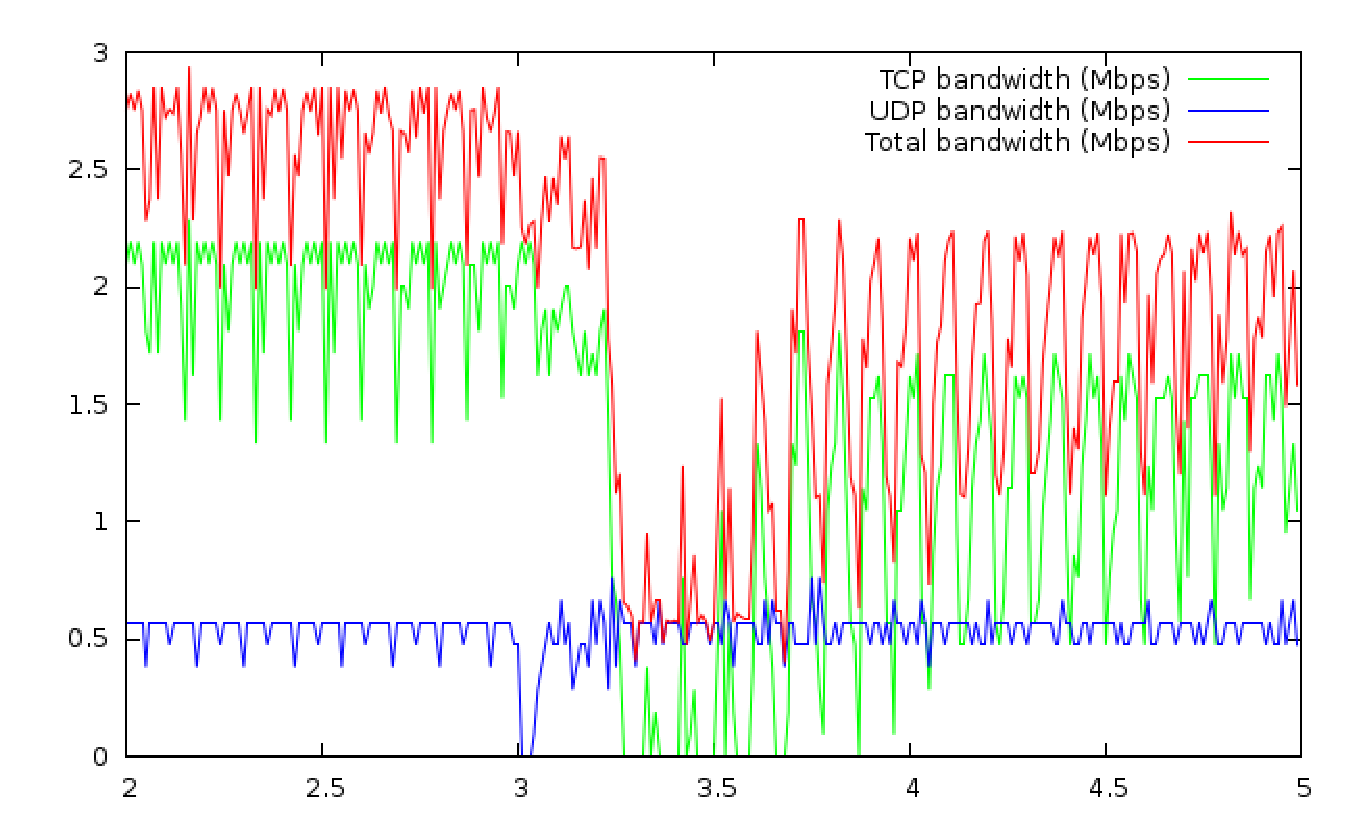
\includegraphics[width=\textwidth]{question1/Q1_6.eps}
    \end{center}

    \paragraph{}All along the simulation, we can see TCP Tahoe running its
congestion-avoidance algorithm. \newline
Soon after 3.0 sec, when the n0 to n2 link falls down, TCP reinitialized its
sending window and its congestion-detection algorithm. As said in
\ref{Network recovery}, TCP recovered an ideal throughput shortly after 3.5 sec
and correctly took into account the new UDP traffic on the n0 to n1 link.

    \paragraph{}After the traffic has been redirected on the n0 to n1
link, this last becomes a bottleneck in the network as the total throughput is
approximately 5 Mbps, the bandwidth of the link.

    \paragraph{}The script can be run with this command :
    \begin{verbatim}
        runhaskell Q1_6.hs < Q1_3.tr | gnuplot --persist
    \end{verbatim}

  \section{Question 2}

    \subsection{RDV point selection}

    \paragraph{}The fifth node is at the center of the network and thus is a
good choice for a rendez-vous point.
However from an empirical point of view, the second node is a better choice
because even if there are as many hops to reach nodes 8, 10 and 11, the eighth
node is closer to the second node than the fifth one and is the largest
\enquote{customer} (longer alive) of the multicast group.

  \subsection{Number of hops from n9}

   \subsubsection{Unicast}

    \paragraph{}The following table gives the minimum number of hops needed to
reach n8, n10 and n11 from n9.

    \begin{center}
            \begin{tabular}{|l|l|l|}
                \hline
                From & To & \# of hops \\
                \hline
                n9 & n8  & 2 \\
                n9 & n10 & 2 \\
                n9 & n11 & 4 \\
                \hline
            \end{tabular}
    \end{center}

   \subsubsection{Sparse mode}

    \paragraph{}Packets take two hops to go to the n5 RDV point and then one
hops to reach n8, n10 and n11 from n5. Thus n8, n10 and n11 are each 4 hops
away from n9\footnote{The RDV point has been accounted as an additional hop.} in
this multicast configuration. This is less efficient in number of hops than
using unicast but it saves the n0 to n1 and n1 to n2 links by avoiding
duplicates.

   \subsubsection{Dense mode}

    \paragraph{}In dense mode, the protocol succeeds to learn the shortest
paths for each of the three destinations, thus the number of crossed hops is
the same as in the unicast mode.

    \paragraph{}When the dense mode has been stabilized, the way packets are
transmitted is optimal, as every packets take the shortest path (by contrast to
the sparse mode) and there is no duplicate on a single link (by contrast the
unicast scenario).
\newline However there is a stabilization overhead as the default router policy
is to broadcast multicast packets before receiving a prune.

  \subsection{Prunes and grafts}

    \begin{center}
        \begin{tabular}{|l|l|l|}
            \hline
            Mode   & \# of prunes & \# of grafts \\
            \hline
            Sparse & 197          & 8 \\
            Dense  & 2260         & 14 \\
            \hline
        \end{tabular}
    \end{center}

    \paragraph{}In sparse mode, grafts are sent when a node needs to join the
group (8 grafts because 2 grafts are needed for each of the 4 joins, as
there is an additional router from each node to n5).
\newline Prunes are sent when a node leaves the group (the number is quite huge
because multiple prunes are sent before being propagated in the network).

    \paragraph{}In dense mode, a lot of prunes are sent during the network
stabilization (because of the default policy to propagate packets in every
routers). Grafts are only sent when a node joins the group. Grafts are propagated
in the whole network and are so more numerous than in the sparse mode
simulation.

    \paragraph{}The script can be run with these commands :
    \begin{verbatim}
        runhaskell Q2_3.hs < Q2_1_sparse.tr
        runhaskell Q2_3.hs < Q2_1_dense.tr
    \end{verbatim}

  \subsection{FTP flow}

    \paragraph{}The FTP flow has not any consequence on the sparse simulation as
they do not use any link in common.

    \paragraph{}However in the dense simulation, the default broadcast policy
has an undesirable side-effect on the TCP flow : the sudden yet short increase
in traffic generates some packet loss and resets the congestion control
algorithm. This implies a noticeable decline in the TCP throughput :
\newline In sparse mode, the TCP throughput is equal to 3.3 Mbps whereas it is
only of 2.2 Mbps in the dense simulation.

    \paragraph{}The script can be run with these commands :
    \begin{verbatim}
        runhaskell Q2_4.hs < Q2_4_sparse.tr
        runhaskell Q2_4.hs < Q2_4_dense.tr
    \end{verbatim}

  \subsection{UDP flow}

    \paragraph{}The aggressive UDP flow creates buffer overflows in n6.
Sometimes, it can result in a unpredictable loss of the graft packet, as in
the sparse simulation.

    \paragraph{}This problem could be avoided by implementing a reliable
graft protocol, by notifying the sender of the delivery of the graft.

  \subsection{Dense mode or Sparse mode}
	 \paragraph{} First, we can say that the dense mode is better in a small network. It is due to the fact that packets do not have to reach the RDV point (the network's traffic is decentralized). Thus, there is less bandwidth needed because packets go directly to their recievers but it has a stabilization time. Furthermore, dense mode is better when multiple routers want to be in the group (Sparse mode can assume, relatively, just a few revievers). Opposed to those advantages, the dense mode re-flood  the multicast traffic periodically so it uses some bandwidth and could cause trouble. Here, the dense mode is obviously more convenient.

	\paragraph{} Secondly, the sparse mode is quite different for multicasting because it uses an explicit request approach. Thus, the traffic is more ordered and so, a larger amount of data could be sent. This mode suits better for a bigger network with more than 12 nodes. Moreover, the RDV point have to deal with a very high amount of data but those packets only go directly where they are needed. So it leaves certain routers alone which do not have to treat those packets.

\end{document}
